\documentclass[preview]{standalone}
%graphics
\usepackage{tikz}
\usetikzlibrary{arrows.meta,math,calc}

\usepackage{subfig}
\definecolor{cs1}{RGB}{89,89,91}
\definecolor{cs2}{RGB}{129,130,132}
\definecolor{cs3}{RGB}{210,210,212}
\definecolor{cs4}{RGB}{168,169,173}
\definecolor{inp}{RGB}{230,230,230}
\definecolor{out}{RGB}{40,40,40}
\definecolor{fix}{RGB}{0,0,0}
\begin{document}
  
  \tikzstyle{c}=[rectangle, fill, text=black, minimum size=1cm]
  \tikzstyle{c1}=[lightgray!50, c]
  \tikzstyle{c2}=[lightgray, c] 
  \tikzstyle{c3}=[gray, c]
  \tikzstyle{c4}=[darkgray!90, c]
  
  \begin{figure}[!t]
    
    \centering
    \subfloat[A* path finding]{
      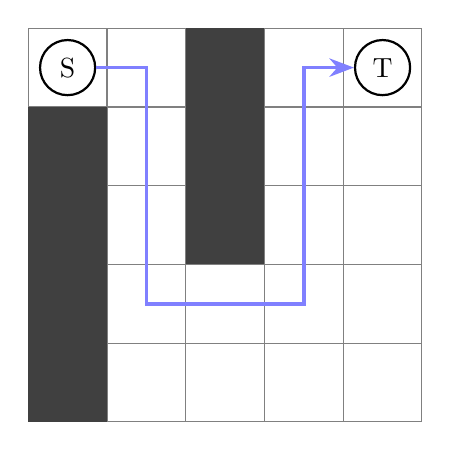
\begin{tikzpicture}[
        %x={(2cm, 0cm)},
        y={(0cm,-1cm)},
        %scale=.6,transform shape,
        v/.style={circle, draw, fill=white, line width = 0.8pt, minimum size=.7cm},
        obs/.style={rectangle, fill, darkgray, minimum size=1cm},
        route/.style={->, >={Stealth[]},line width=1.3pt, blue!50},
        ]
        
        \foreach \x in {0,1,2,3,4}
        \foreach \y in {0,1,2,3,4} {
          \draw[gray] (\x,\y) +(-.5,-.5) rectangle ++(.5,.5);
        }
        \node(start) [v] at (0,0) {S};
        \node(target)[v] at (4,0) {T};
        \node(obs1)[obs] at (0,1){};
        \node(obs2)[obs] at (0,2){};
        \node(obs3)[obs] at (0,3){};
        \node(obs4)[obs] at (0,4){};
        \node(obs5)[obs] at (2,0){};
        \node(obs6)[obs] at (2,1){};
        \node(obs7)[obs] at (2,2){};
        \node(obs8)[obs] at (0,1){};
        
        \draw[route](start)-|(1,3)--(3,3)|-(target.west);
        
      \end{tikzpicture}
    }
    \hfil
    \subfloat[A* on USE clocking scheme]{
      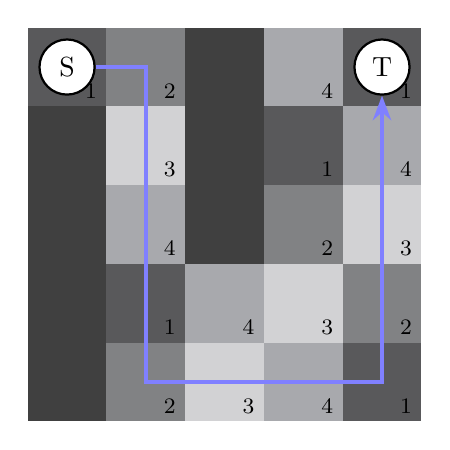
\begin{tikzpicture}[
        y={(0cm,-1cm)},
        c1/.style={shape=rectangle, fill=cs1, text=black, minimum size=1cm},
        c2/.style={shape=rectangle, fill=cs2, text=black, minimum size=1cm},
        c3/.style={shape=rectangle, fill=cs3, text=black, minimum size=1cm},
        c4/.style={shape=rectangle, fill=cs4, text=black, minimum size=1cm},
        v/.style={circle, draw, fill=white, line width = 0.8pt, minimum size=.7cm},
        obs/.style={rectangle, fill, darkgray, minimum size=1cm},
        route/.style={->, >={Stealth[]},line width=1.3pt, blue!50},
        ]
        \tikzmath{
          function use(\x,\y){
            return (mod(\y,2)!=0) ? 
            ((mod(\y+1,4)!=0)?(4-mod(\x,4)):(4-mod(\x+2,4))) :
            ((mod(\y,4)==0)?(1+mod(\x,4)):(1+mod(\x+2,4)));
          };
          %
          int \i, \j, \c; 
          for \i in {0,1,2,3,4}{
            for \j in {0,1,2,3,4}{
              \c = use(\i,\j);
              {
                \path 
                (\i,\j)                                node(\i\j)[c\c]{}
                ($(\i\j.center)!.6!(\i\j.south east)$) node{\footnotesize \c};
              };
            };
          };
        }     
        \node(start) [v] at (0,0) {S};
        \node(target)[v] at (4,0) {T};
        \node(obs1)[obs] at (0,1){};
        \node(obs2)[obs] at (0,2){};
        \node(obs3)[obs] at (0,3){};
        \node(obs4)[obs] at (0,4){};
        \node(obs5)[obs] at (2,0){};
        \node(obs6)[obs] at (2,1){};
        \node(obs7)[obs] at (2,2){};
        \node(obs8)[obs] at (0,1){};
        
        \draw[route](start)-|(1,4)-|(target.south);
      \end{tikzpicture}
    }
  \end{figure}
\end{document}
